%Master File:lectures.tex

\lesson{Writing an Arrays}

\vspace*{-2cm}
\begin{center}
  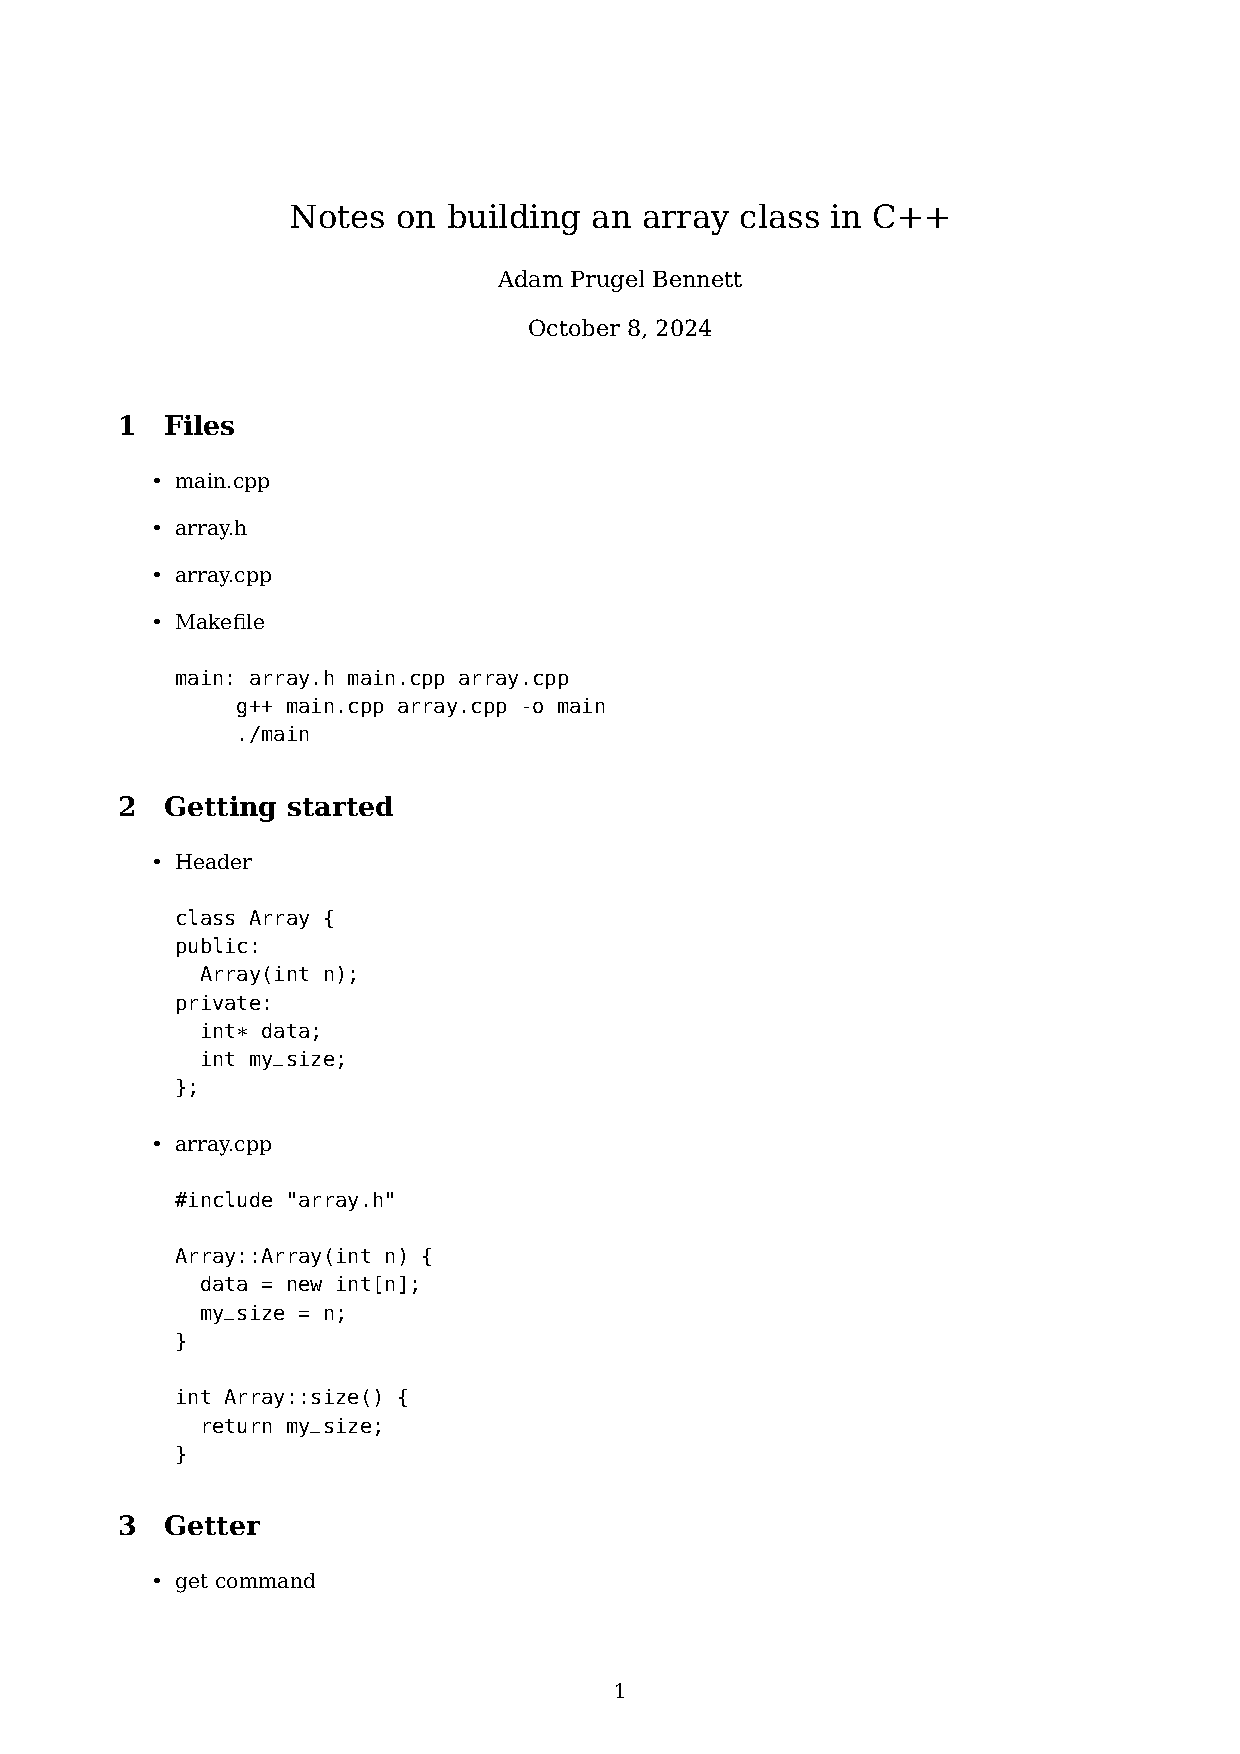
\includegraphics[height=11cm]{array}
\end{center}
\vspace*{-1cm}
\keywords{Resizeable arrays, iterators}

%%%%%%%%%%%%%%%%%%%%%%% Next Slide %%%%%%%%%%%%%%%%%%%%%%%

\begin{slide}
\section[-2]{Resizable Arrays}

\begin{itemize}
\item We are finally in a position where we can make our array
  resizable
\item We need to have both a length (which the user know about) and a
  capacity which is invisible to the user, but allows us to add
  elements while not having to create too many new arrays
\item We need to change the constructor
  \begin{cpp}
  template <typename T>
  Array<T>::Array(unsigned n=0) {
    length = n;
    if (n==0) {
      n = 8;
    }
    data = new T[n];
    capacity = n;
  }
  \end{cpp}
\item If we don't give the constructor an argument it will be set to 0
\end{itemize}
\end{slide}

%%%%%%%%%%%%%%%%%%%%%%% Next Slide %%%%%%%%%%%%%%%%%%%%%%%

\begin{slide}
  \section[-2]{Push Back}
  
  \begin{itemize}
  \item Let's introduce a new command that allows us to add to the end
    of an array
  \item If the capacity is not big enough we need to increase the
    capacity
    \begin{cpp}
template <typename T>
T Array<T>::push_back(T value) {
  if (length == capacity) {
    capacity *= 2;
    T* new_data = new T[capacity];
    for (int i=0; i<length; ++i) {
      new_data[i] = data[i];
    }
    delete [] data;
    data = new_data;
  }
  data[length] = value;
  ++length;
  return value;
}
    \end{cpp}
  \end{itemize}
\end{slide}

%%%%%%%%%%%%%%%%%%%%%%% Next Slide %%%%%%%%%%%%%%%%%%%%%%%

\begin{slide}
\section{Refactoring}

\begin{PauseHighLight}
  \begin{itemize}
  \item It is possible to define functions inside the class definition
  \item This has the advantage of making the code much more compact
  \item It has the disadvantage of confusing the interface (a list of
    function that can be called) with the implementation
  \item It is unfortunate that when you use templates you tend to put
    the implementation details in the header file
  \item What you should do depend on whether you are after a quick
    solution or are writing code that many people might use
  \end{itemize}
\end{PauseHighLight}

\end{slide}

%%%%%%%%%%%%%%%%%%%%%%% Next Slide %%%%%%%%%%%%%%%%%%%%%%%

\begin{slide}
\section[-2]{New Code}

\begin{cpp}
template <typename T>
class Array {
private:
  T *data;
  unsigned length;
  unsigned capacity;
public:
  Array(unsigned n=0) {
    length = n;
    if (n==0) {
      n = 8;
    }
    data = new T[n];
    capacity = n;
  }
  Array(const Array& other);
  ~Array() {delete[] data;}
  T& operator[](unsigned index) {return data[index];}
  const T& operator[](unsigned index) const {return data[index];}
  unsigned size() const {return length;}
  T push_back(T value);
};
\end{cpp}

\end{slide}

%%%%%%%%%%%%%%%%%%%%%%% Next Slide %%%%%%%%%%%%%%%%%%%%%%%

\begin{slide}
\section{Iterators}

\begin{PauseHighLight}
  \begin{itemize}
  \item Iterators are designed to follow the same semantics as
    pointers
  \item Because we are just wrapping an array where we can use
    pointers to navigate the array we can use pointers as iterators
  \item All we need to do is add two new methods
    \begin{cpp}
        T* begin() {return data;}
        T* end() {return data+length;}
    \end{cpp}
  \item We can the use iterators to iterate over our array
  \end{itemize}
\end{PauseHighLight}

\end{slide}


%%%%%%%%%%%%%%%%%%%%%%% Next Slide %%%%%%%%%%%%%%%%%%%%%%%

\begin{slide}
\section{vector}

\begin{itemize}
\item C++ comes with a powerful library known as the \emph{standard
    template library} (STL)
\item This includes containers (resizable arrays, linked lists, double
  ended queues, sets, maps, etc.)
\item The resizable array is called \texttt{vector<T>}
\item We can just replace \texttt{"array.h"} with \texttt{<vector>}
  and \texttt{Array} with \texttt{vector} in our main function and
  everything will work the same
\item Of course the STL vector is a bit more powerful and efficient
  than the \texttt{Array} class we wrote, although our class isn't bad
\end{itemize}

\end{slide}

%%%%%%%%%%%%%%%%%%%%%%% Next Slide %%%%%%%%%%%%%%%%%%%%%%%

\begin{slide}
\section{Iterators in Other Containers}

\begin{PauseHighLight}
  \begin{itemize}
  \item Iterators exist for many containers
  \item Because of iterators it is possible to write algorithms that
    work for any container that supports iterators
  \item The STL has a bunch of algorithms that work for different
    containers
  \item You can also use a pretty for loop
    \begin{cpp}
      for(T entry: container) {
        ...
      }
    \end{cpp}
  \item This makes code easier to read
  \end{itemize}
\end{PauseHighLight}

\end{slide}

%%%%%%%%%%%%%%%%%%%%%%% Next Slide %%%%%%%%%%%%%%%%%%%%%%%

\begin{slide}
\section{Writing Iterators}

\begin{PauseHighLight}
  \begin{itemize}
  \item For most classes we don't iterator by advancing a pointer
  \item Thus most iterators are more complex and we have to write a
    class (or structure---\texttt{struct}) which keeps the information
    we need to iterate 
  \item We then have to define methods to make iteration look like
    iterating though an array
  \item We will see an example in the code for linked lists
  \end{itemize}
\end{PauseHighLight}

\end{slide}
